% Created by tikzDevice version 0.12.3.1 on 2022-09-02 16:29:44
% !TEX encoding = UTF-8 Unicode
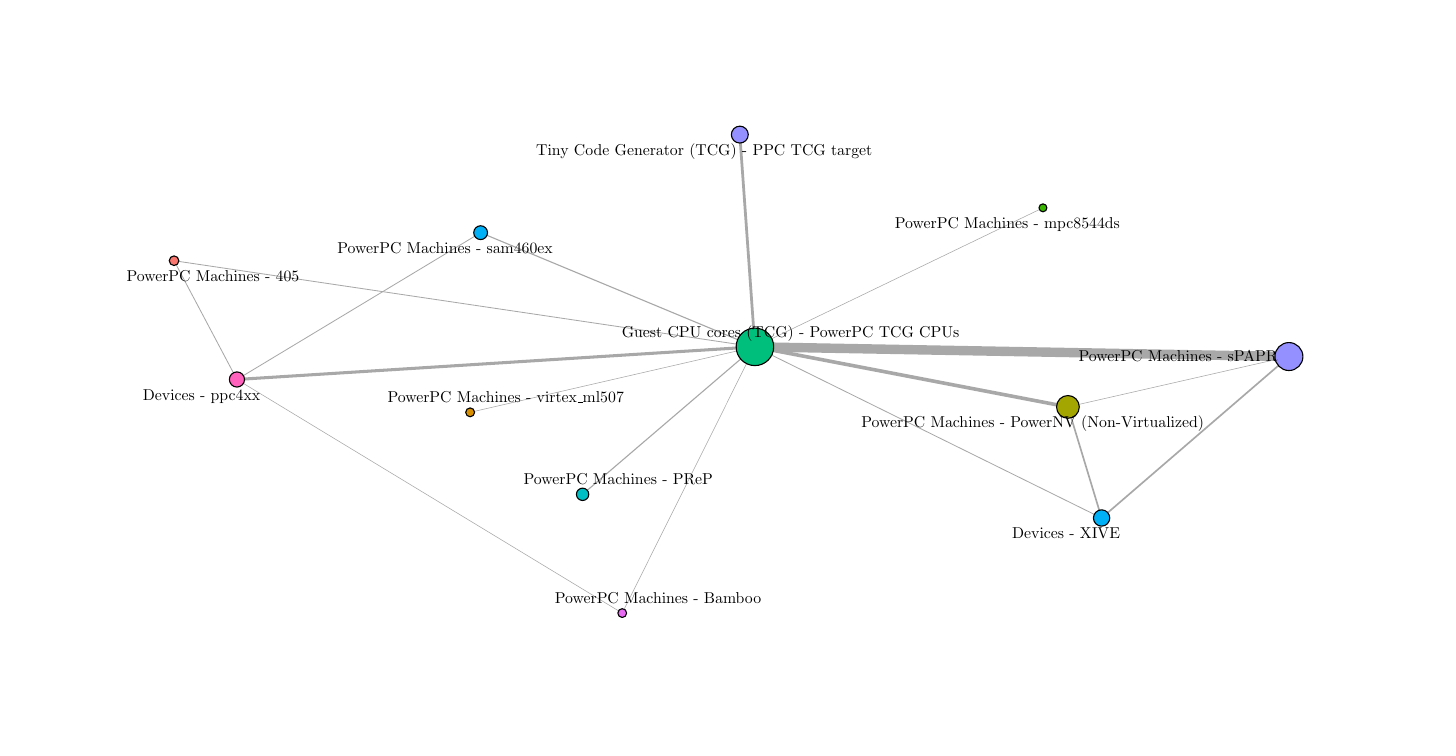
\begin{tikzpicture}[x=1pt,y=1pt]
\definecolor{fillColor}{RGB}{255,255,255}
\path[use as bounding box,fill=fillColor,fill opacity=0.00] (0,0) rectangle (505.89,252.94);
\begin{scope}
\path[clip] (  0.00,  0.00) rectangle (505.89,252.94);
\definecolor{fillColor}{RGB}{255,255,255}

\path[fill=fillColor] (  0.00,  0.00) rectangle (505.89,252.94);
\end{scope}
\begin{scope}
\path[clip] ( 32.75, 32.75) rectangle (475.89,222.94);
\definecolor{drawColor}{gray}{0.66}

\path[draw=drawColor,line width= 0.3pt,line join=round] (388.06, 75.76) -- (262.79,137.61);

\path[draw=drawColor,line width= 0.6pt,line join=round] (388.06, 75.76) -- (375.89,115.90);

\path[draw=drawColor,line width= 0.6pt,line join=round] (388.06, 75.76) -- (455.75,134.10);

\path[draw=drawColor,line width= 1.1pt,line join=round] ( 75.62,125.81) -- (262.79,137.61);

\path[draw=drawColor,line width= 0.3pt,line join=round] ( 75.62,125.81) -- ( 52.89,168.73);

\path[draw=drawColor,line width= 0.2pt,line join=round] ( 75.62,125.81) -- (214.84, 41.40);

\path[draw=drawColor,line width= 0.3pt,line join=round] ( 75.62,125.81) -- (163.67,178.86);

\path[draw=drawColor,line width= 0.3pt,line join=round] (262.79,137.61) -- ( 52.89,168.73);

\path[draw=drawColor,line width= 0.2pt,line join=round] (262.79,137.61) -- (214.84, 41.40);

\path[draw=drawColor,line width= 0.4pt,line join=round] (262.79,137.61) -- (200.52, 84.32);

\path[draw=drawColor,line width= 1.3pt,line join=round] (262.79,137.61) -- (375.89,115.90);

\path[draw=drawColor,line width= 0.2pt,line join=round] (262.79,137.61) -- (366.87,187.84);

\path[draw=drawColor,line width= 3.4pt,line join=round] (262.79,137.61) -- (455.75,134.10);

\path[draw=drawColor,line width= 0.4pt,line join=round] (262.79,137.61) -- (163.67,178.86);

\path[draw=drawColor,line width= 0.2pt,line join=round] (262.79,137.61) -- (159.88,113.94);

\path[draw=drawColor,line width= 1.0pt,line join=round] (262.79,137.61) -- (257.33,214.30);

\path[draw=drawColor,line width= 0.2pt,line join=round] (375.89,115.90) -- (455.75,134.10);
\definecolor{drawColor}{RGB}{0,0,0}
\definecolor{fillColor}{RGB}{0,176,246}

\path[draw=drawColor,line width= 0.4pt,line join=round,line cap=round,fill=fillColor] (388.06, 75.76) circle (  2.95);
\definecolor{fillColor}{RGB}{255,98,188}

\path[draw=drawColor,line width= 0.4pt,line join=round,line cap=round,fill=fillColor] ( 75.62,125.81) circle (  2.74);
\definecolor{fillColor}{RGB}{0,191,125}

\path[draw=drawColor,line width= 0.4pt,line join=round,line cap=round,fill=fillColor] (262.79,137.61) circle (  6.78);
\definecolor{fillColor}{RGB}{248,118,109}

\path[draw=drawColor,line width= 0.4pt,line join=round,line cap=round,fill=fillColor] ( 52.89,168.73) circle (  1.74);
\definecolor{fillColor}{RGB}{231,107,243}

\path[draw=drawColor,line width= 0.4pt,line join=round,line cap=round,fill=fillColor] (214.84, 41.40) circle (  1.59);
\definecolor{fillColor}{RGB}{0,191,196}

\path[draw=drawColor,line width= 0.4pt,line join=round,line cap=round,fill=fillColor] (200.52, 84.32) circle (  2.23);
\definecolor{fillColor}{RGB}{163,165,0}

\path[draw=drawColor,line width= 0.4pt,line join=round,line cap=round,fill=fillColor] (375.89,115.90) circle (  4.11);
\definecolor{fillColor}{RGB}{57,182,0}

\path[draw=drawColor,line width= 0.4pt,line join=round,line cap=round,fill=fillColor] (366.87,187.84) circle (  1.43);
\definecolor{fillColor}{RGB}{149,144,255}

\path[draw=drawColor,line width= 0.4pt,line join=round,line cap=round,fill=fillColor] (455.75,134.10) circle (  5.05);
\definecolor{fillColor}{RGB}{0,176,246}

\path[draw=drawColor,line width= 0.4pt,line join=round,line cap=round,fill=fillColor] (163.67,178.86) circle (  2.49);
\definecolor{fillColor}{RGB}{216,144,0}

\path[draw=drawColor,line width= 0.4pt,line join=round,line cap=round,fill=fillColor] (159.88,113.94) circle (  1.60);
\definecolor{fillColor}{RGB}{149,144,255}

\path[draw=drawColor,line width= 0.4pt,line join=round,line cap=round,fill=fillColor] (257.33,214.30) circle (  3.05);

\node[text=drawColor,anchor=base,inner sep=0pt, outer sep=0pt, scale=  0.57] at (375.24, 68.28) {Devices - XIVE};

\node[text=drawColor,anchor=base,inner sep=0pt, outer sep=0pt, scale=  0.57] at ( 62.82,118.33) {Devices - ppc4xx};

\node[text=drawColor,anchor=base,inner sep=0pt, outer sep=0pt, scale=  0.57] at (275.69,141.15) {Guest CPU cores (TCG) - PowerPC TCG CPUs};

\node[text=drawColor,anchor=base,inner sep=0pt, outer sep=0pt, scale=  0.57] at ( 66.96,161.24) {PowerPC Machines - 405};

\node[text=drawColor,anchor=base,inner sep=0pt, outer sep=0pt, scale=  0.57] at (227.77, 44.99) {PowerPC Machines - Bamboo};

\node[text=drawColor,anchor=base,inner sep=0pt, outer sep=0pt, scale=  0.57] at (213.41, 87.91) {PowerPC Machines - PReP};

\node[text=drawColor,anchor=base,inner sep=0pt, outer sep=0pt, scale=  0.57] at (363.14,108.44) {PowerPC Machines - PowerNV (Non-Virtualized)};

\node[text=drawColor,anchor=base,inner sep=0pt, outer sep=0pt, scale=  0.57] at (354.03,180.35) {PowerPC Machines - mpc8544ds};

\node[text=drawColor,anchor=base,inner sep=0pt, outer sep=0pt, scale=  0.57] at (415.70,132.18) {PowerPC Machines - sPAPR};

\node[text=drawColor,anchor=base,inner sep=0pt, outer sep=0pt, scale=  0.57] at (150.85,171.38) {PowerPC Machines - sam460ex};

\node[text=drawColor,anchor=base,inner sep=0pt, outer sep=0pt, scale=  0.57] at (172.75,117.52) {PowerPC Machines - virtex{\_{}}ml507};

\node[text=drawColor,anchor=base,inner sep=0pt, outer sep=0pt, scale=  0.57] at (244.48,206.81) {Tiny Code Generator (TCG) - PPC TCG target};
\end{scope}
\end{tikzpicture}
